[12~v\textsuperscript{o}] Genesis autem seriei prioris, cum scilicet vis\protect\index{Sachverzeichnis}{vis} aequabilis esse ponatur, ita brevissime enuntiari \edtext{potest: Terminus seriei quilibet ducatur in quantitatem}{\lemma{potest:}\Bfootnote{\textit{(1)}\ quantitas \textit{(2)}\ Terminus  \textit{(a)}\ progressionis quilibet \textit{(b)}\ seriei [...] quantitatem \textit{L}}} constantem $\rule[-4mm]{0mm}{10mm}\displaystyle \edtext{\frac{b}{r}$, factus}{\lemma{$\displaystyle \frac{b}{r}$,}\Bfootnote{\textit{(1)}\ productu \textit{(2)}\ factus \textit{L}}} ab ipso termino auferatur, residuum erit terminus sequens.
\pend
\newpage
%\vspace{1.5em}
%\pstart
%\noindent
%\centering
%     %\begin{wrapfigure}{l}{0.4\textwidth}
%     %\vspace*{-4mm}
%     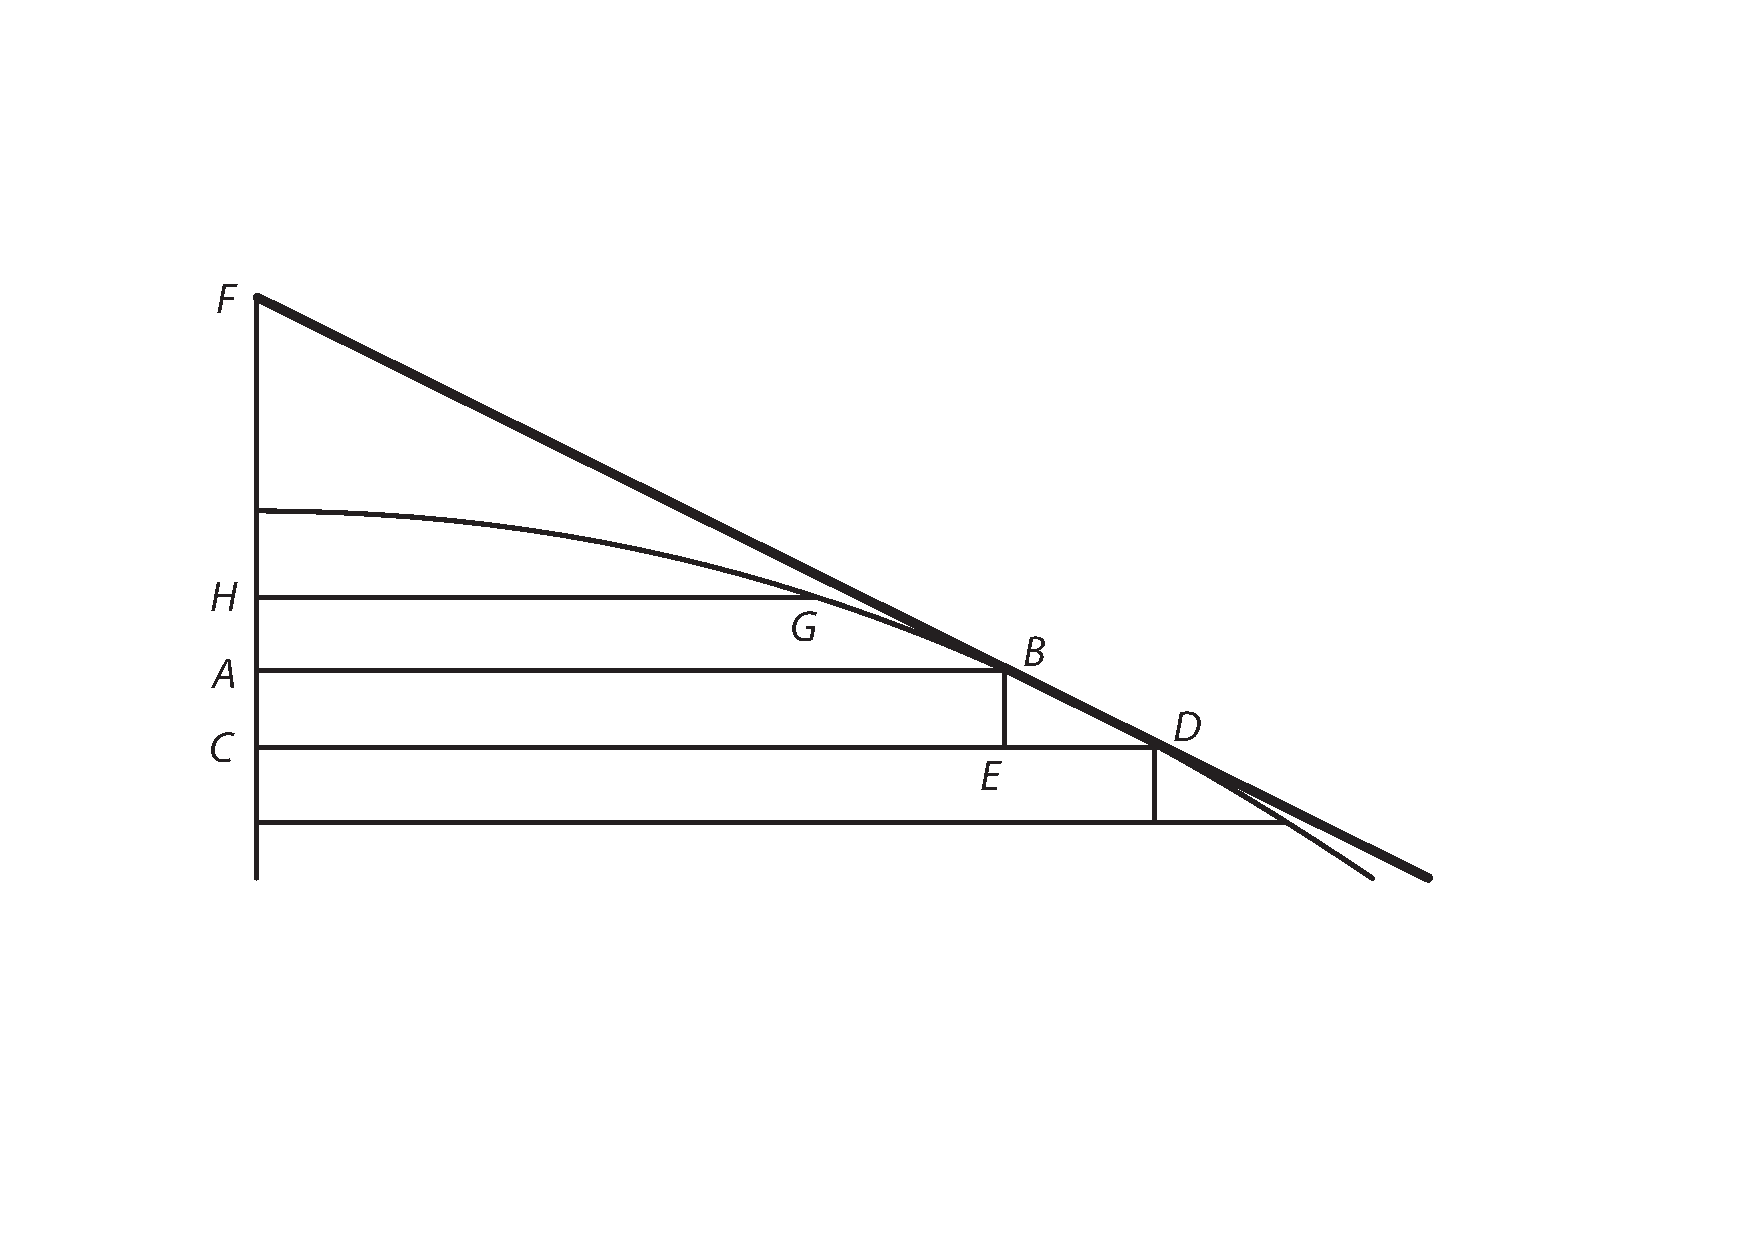
\includegraphics[trim = 0mm -3mm 0mm 0mm, clip, width=0.7\textwidth]{images/lh03705_012v_1-d1.pdf}\\ 
%    \noindent \centering  [\textit{Fig. 2}] % \caption{Bildbeschreibung}
%     %\end{wrapfigure}
%\pend
\pstart
$\rule[-4mm]{0mm}{10mm}\displaystyle$Ex linea $CD$ quaeratur linea $AB$. Nempe $\rule[-4mm]{0mm}{10mm}\displaystyle \frac{ED}{\beta \sqcap BE} \, \sqcap \, \frac{CD}{CF}$. Ergo $\rule[-4mm]{0mm}{10mm}\displaystyle ED \, \sqcap \, \frac{CD \beta}{CF}$. Jam $AB \, \sqcap \, CD - ED$. Ergo $\rule[-4mm]{0mm}{10mm}\displaystyle AB \, \sqcap \, CD - \frac{CD}{CF}\beta$ $\rule[-4mm]{0mm}{10mm}\displaystyle \ovalbox{sive $\displaystyle\frac{AB}{CD} \sqcap \frac{CF - \beta}{CF}$}\,$. Jam in nostro casu $\rule[-4mm]{0mm}{10mm}\displaystyle AB \, \sqcap \, CD - \frac{b}{r} \, CD$. Ergo $\rule[-4mm]{0mm}{10mm}\displaystyle \frac{\beta}{CF} \sqcap \frac{b}{r}$. Erit ergo $CF$ linea constans $\rule[-4mm]{0mm}{10mm}\displaystyle \sqcap \frac{r \beta}{b}$. \edtext{$\displaystyle HG \, \sqcap \, AB, \smallfrown 1 - \frac{b}{r}$ et $\displaystyle AB \, \sqcap \, CD, \smallfrown 1 - \frac{b}{r}$. Ergo $\displaystyle HG \, \sqcap \, CD, \smallfrown 1 - \frac{2b}{r} + \frac{b^2}{r^2}$.}{\lemma{}\Bfootnote{$\displaystyle HG \, \sqcap \, AB, \smallfrown $ [...] $\displaystyle + \frac{b^2}{r^2}$. \textit{erg.} \textit{L}}}$\rule[-4mm]{0mm}{10mm}\displaystyle$ Unde illud quoque necessario concluditur ipsam $b$ esse infinite parvam, alioqui enim statim antequam per spatium continuum quantulumcunque vis progredi posset, exhauriri motum. Idque ex calculo patet. Nam $CF$ necesse est esse lineam non infinite parvam sed ordinariam, jam $\beta$ est infinite parva; ergo \edtext{etiam $b$}{\lemma{etiam}\Bfootnote{\textit{(1)}\ $\beta$ \textit{(2)}\ $b$ \textit{L}}} dividens erit infinite parva ut eam tollat, et fiat $\rule[-4mm]{0mm}{10mm}\displaystyle CF \sqcap \frac{r \beta}{b} \sqcap \rule[-4mm]{0mm}{10mm}\displaystyle \frac{rb}{b} \sqcap r$.
Jam cum $CF$ non minus quam $BE$ sit semper linea constans, hinc porro sequitur quae est ratio ipsius differentiae $ED$, ad lineam constantem $BE$, eam etiam esse ipsius ordinatae $CD$ ad lineam constantem $CF$. Ergo eadem perpetuo erit ratio differentiarum ad ordinatas; quia\hfill eadem\hfill perpetuo\hfill ratio\hfill est\hfill $CF$\hfill ad\hfill $BE$.\hfill Ergo\hfill progressio\hfill tam\hfill ordinatarum\hfill quam differentiarum Geometrica est. Ac proinde linea $GBD$ est logarithmica. Itaque si \edtext{vires relictae a detritu}{\lemma{vires}\Bfootnote{\textit{(1)}\ quaesitae \textit{(2)}\ relictae a detritu \textit{L}}} sint ut numeri, spatia percursa\protect\index{Sachverzeichnis}{spatium percursum} erunt ut Logarithmi. En ergo.
\pend
\vspace{1em}
\pstart
\noindent
\centering
     %\begin{wrapfigure}{l}{0.4\textwidth}
     %\vspace*{-4mm}
     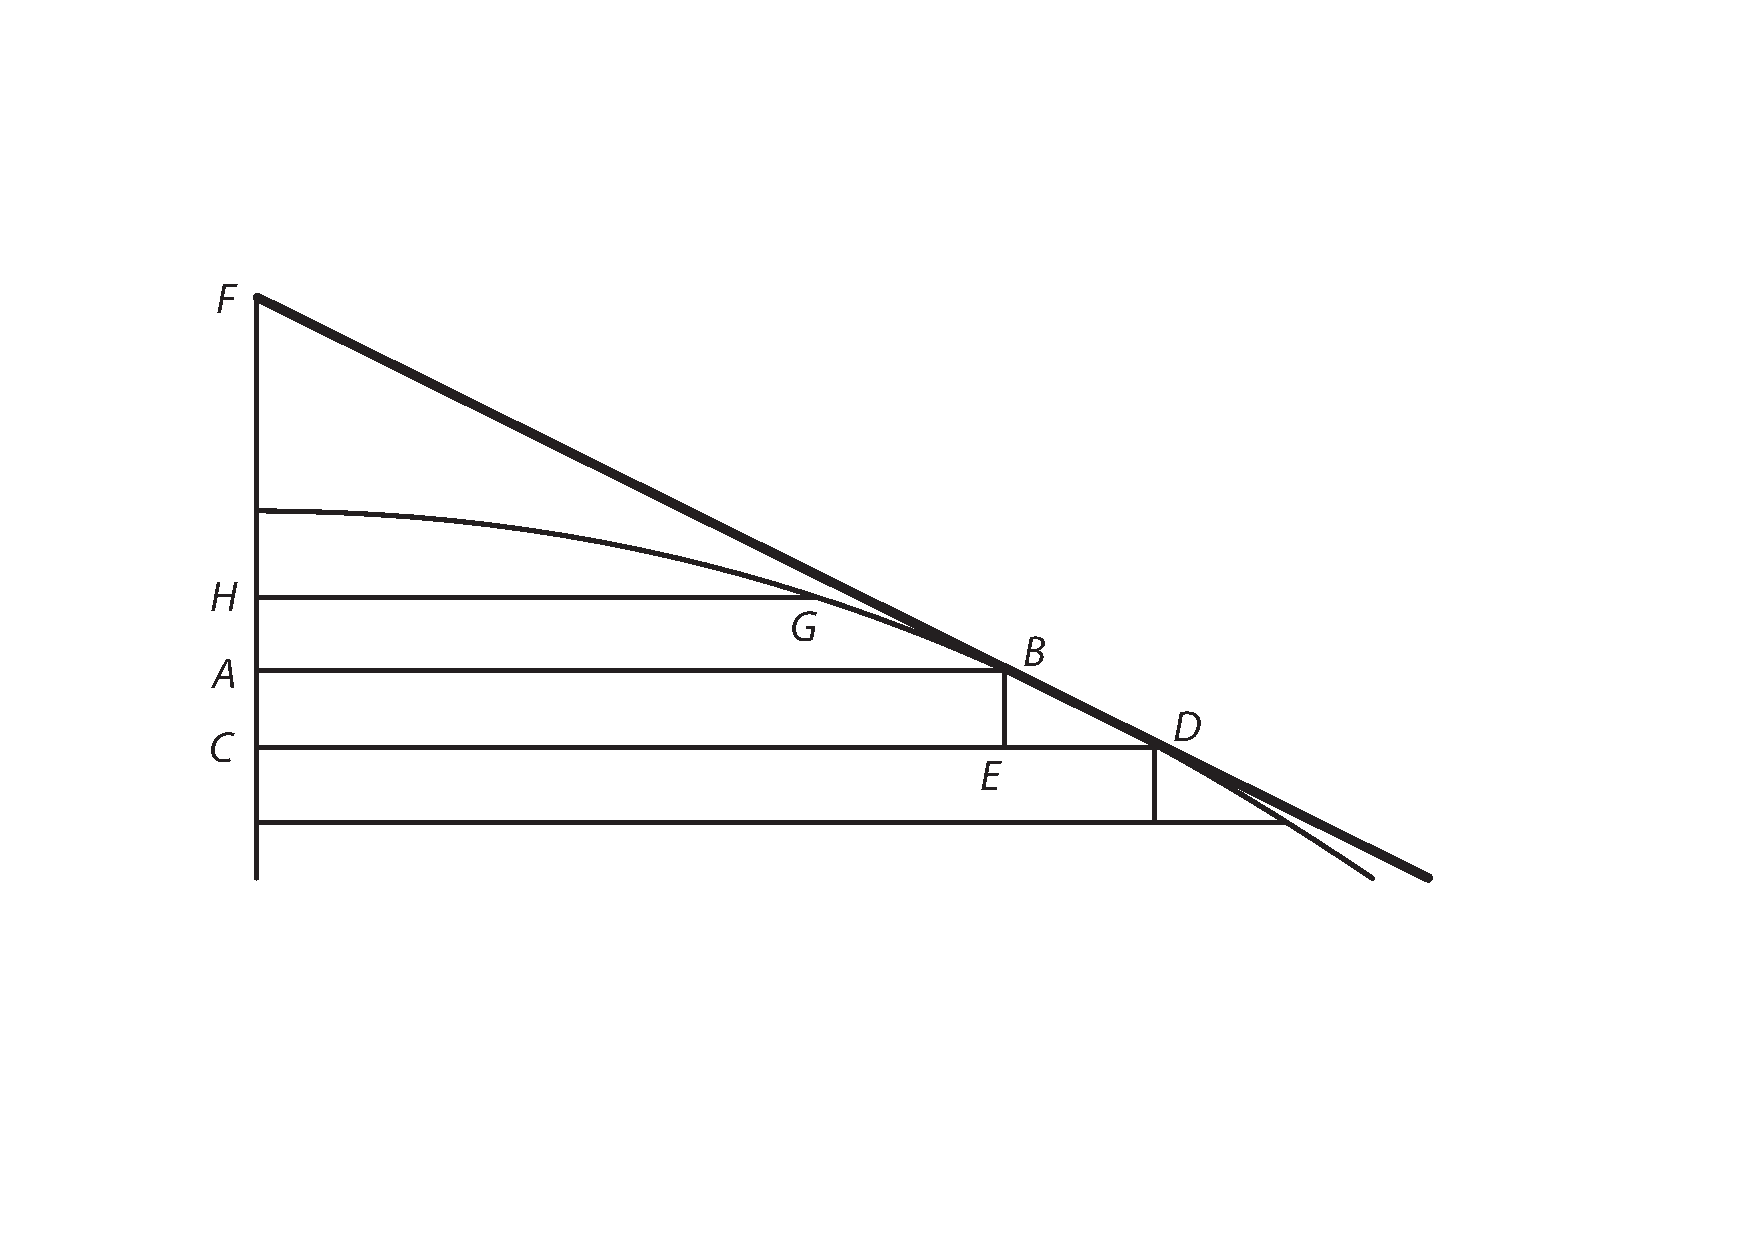
\includegraphics[trim = 0mm -3mm 0mm 0mm, clip, width=0.78\textwidth]{images/lh03705_012v_1-d1.pdf}\\ 
    \setline{1}\noindent \setline{1}\centering  [\textit{Fig. 2}] % \caption{Bildbeschreibung}
     %\end{wrapfigure}
\pend
\count\Afootins=1500
\count\Bfootins=1500
\count\Cfootins=1500
\newpage